\documentclass[pdftex12pt, a4paper]{book}
\usepackage[pdftex]{graphicx}
\usepackage{amsmath}
\usepackage{boxedminipage}
\usepackage{hyperref}
\usepackage{fullpage}
\usepackage{listings}
\usepackage{xcolor}
\usepackage{caption}
%\usepackage[toc]{glossaries}
\usepackage[T1]{fontenc}
\usepackage{float}
\usepackage[parfill]{parskip}
\usepackage{subfigure}
\usepackage{units} % better spacing between value and units
\usepackage{textcomp}
\usepackage[official]{eurosym} % better eurosign
\usepackage{multirow} % for tables
\usepackage{booktabs} % makes tables look better

% Glossary
\usepackage[nomain,acronym,toc,section]{glossaries}
\newglossary{symbol}{sbl}{smb}{Symbols}
\makeglossaries
\usepackage[xindy]{imakeidx}
\makeindex

% Fancy listings
\DeclareCaptionFont{white}{\color{white}}
\DeclareCaptionFormat{listing}{%
  \parbox{\textwidth}{\colorbox{gray}{\parbox{\textwidth}{#1#2#3}}\vskip-4pt}}
\captionsetup[lstlisting]{format=listing,labelfont=white,textfont=white}
\lstset{frame=lrb,xleftmargin=\fboxsep,xrightmargin=-\fboxsep,language=[LaTeX]{TeX},columns=flexible}
\renewcommand{\lstlistingname}{Snippet}

% Title page stuff
\newcommand{\HRule}{\rule{\linewidth}{0.5mm}}
\renewcommand{\thefigure}{\thesection.\arabic{figure}}
\newcommand{\resetfigurecounter}{\setcounter{figure}{0}}

% Constrain depth in table of contents
\setcounter{tocdepth}{2}

% References
\renewcommand{\bibname}{References}

% Additional commands
\newcommand{\degreeC}{\ensuremath{^\circ}C}
%\newcommand{\unit}[1]{\ensuremath{\, \mathrm{#1}}}

% glossaries
%%% Abbreviations
\newacronym{ccgt}{CCGT}{Combined Cycle Gas Turbine} 
\newacronym{tso}{TSO}{Transmission System Operator}
\newacronym[longplural={Access Responsible Parties}]{arp}{ARP}{Access Responsible Party}
\newacronym[longplural={Balance Responsible Parties}]{brp}{BRP}{Balance Responsible Party}
\newacronym{nrv}{NRV}{Net Regulation Volume}
\newacronym{mip}{MIP}{Marginal Incremental Price}
\newacronym{mdp}{MDP}{Marginal Decremental Price}
\newacronym{entsoe}{ENTSO-E}{European Network of Transmission System Operators for Electricity}
\newacronym{ucte}{UCTE}{Union for the Coordination of the Transmission of Electricity}
\newacronym{vre}{VRE}{Variable Renewable Energy resources}
\newacronym{creg}{CREG}{Commission for the Regulation of the Electricity and Gas - \textit{Commissie voor de Regulering van de Elektriciteit en het Gas}}
\newacronym{hvdc}{HVDC}{High Voltage Direct Current}
\newacronym{chp}{CHP}{Combined Heat and Power}
\newacronym{wkk}{WKK}{Warmtekrachtkoppeling}
\newacronym{fc}{FC}{Frequency Control}

%% Symbols
\newglossaryentry{alpha}% the label
{%
  type=symbol,
  name={\ensuremath{\alpha}},
  description={additional imbalance fee to stimulate the \glspl{arp} to maintain their balance}
}
\newglossaryentry{beta}% the label
{%
  type=symbol,
  name={\ensuremath{\beta}},
  description={additional imbalance fee to stimulate the \glspl{arp} to maintain their balance}
}
%\makeglossaries

\begin{document}
%% Abbreviations
\newacronym{ccgt}{CCGT}{Combined Cycle Gas Turbine} 
\newacronym{tso}{TSO}{Transmission System Operator}
\newacronym[longplural={Access Responsible Parties}]{arp}{ARP}{Access Responsible Party}
\newacronym[longplural={Balance Responsible Parties}]{brp}{BRP}{Balance Responsible Party}
\newacronym{nrv}{NRV}{Net Regulation Volume}
\newacronym{mip}{MIP}{Marginal Incremental Price}
\newacronym{mdp}{MDP}{Marginal Decremental Price}
\newacronym{entsoe}{ENTSO-E}{European Network of Transmission System Operators for Electricity}
\newacronym{ucte}{UCTE}{Union for the Coordination of the Transmission of Electricity}
\newacronym{vre}{VRE}{Variable Renewable Energy resources}
\newacronym{creg}{CREG}{Commission for the Regulation of the Electricity and Gas - \textit{Commissie voor de Regulering van de Elektriciteit en het Gas}}
\newacronym{hvdc}{HVDC}{High Voltage Direct Current}
\newacronym{chp}{CHP}{Combined Heat and Power}
\newacronym{wkk}{WKK}{Warmtekrachtkoppeling}
\newacronym{fc}{FC}{Frequency Control}

%% Symbols
\newglossaryentry{alpha}% the label
{%
  type=symbol,
  name={\ensuremath{\alpha}},
  description={additional imbalance fee to stimulate the \glspl{arp} to maintain their balance}
}
\newglossaryentry{beta}% the label
{%
  type=symbol,
  name={\ensuremath{\beta}},
  description={additional imbalance fee to stimulate the \glspl{arp} to maintain their balance}
}
\renewcommand{\thepage}{\roman{page}}

\setlength\parindent{0pt}

\begin{titlepage}
\begin{center}


\includegraphics[width=0.5\textwidth]{Images/Sedes}\\[0.1cm]    

\textsc{\LARGE Katholieke Universiteit Leuven}\\[1.5cm]

\HRule \\[0.4cm]
{ \huge \bfseries Thesis \\ \vspace{2mm}Optimal operation of decentralized CHP under uncertainties }\\[0.4cm]

\HRule \\[1.5cm]

\begin{minipage}{0.4\textwidth}
\begin{flushleft} \large
\emph{Author:}\\
Jef \textsc{Dani\"els}\\
\vspace{40mm}
\end{flushleft}
\end{minipage}
\begin{minipage}{0.4\textwidth}
\begin{flushright} \large
\emph{Professor} \\
Prof. Dr. Ir. W. \textsc{D'haeseleer}\\
\emph{Mentor} \\
J. \textsc{Zapata Riveros }\\
\vspace{30mm}
\end{flushright}
\end{minipage}

\vfill

{\large \today}

\end{center}

\end{titlepage}

\newpage

\tableofcontents

\resetfigurecounter

\newenvironment{abstract}{
    \onehalfspacing%
    \chapter*{\centering Abstract}%
}{\input{General/Abstract.tex}}

\addcontentsline{toc}{chapter}{List of abbreviations and Symbols}
\chapter*{List of abbreviations and symbols}
\printglossary[type=\acronymtype,title=Abbreviations,toctitle=Abbreviations]
\printglossary[type=symbol]

\listoffigures

\listoftables

\chapter{Introduction}
\renewcommand{\thepage}{\arabic{page}}
\setcounter{page}{1}
\glsresetall
\label{c:Introduction}

%Only a few papers can be found about controlling the uncertainty of CHP's. There is [ J. K. Kok, C. J. Warmer
, and I. G. Kamphuis, "PowerMatcher:
Multiagent Control in the Electricity Infrastructure," in
Proc. Fourth
International Joint Conference on Autonomous Agents \& Multi-Agent
Systems, AAMAS'05
, Utrecht, the Netherlands, 2005.
AND G. J. Schaeffer and H. Akkermans, "CRISP: Distributed Intelligence in
Critical Infrastructures for
Sustainable Power - D5
.3 Final Summary
Report", ENK5-CT-2002-00673, July 10, 2006. ]; \cite{Houwing2009}. The first one doesn't quantify the costs, the second and the third quantify the costs, but they remain in the cost sector. None of the papers regarding this subject ever make clear whether it would be interesting to invest in CHP's or not. For this reason, this thesis tries to address this issue by delivering an easy price/kW before under which the CHP price would have to go before it would be interesting to invest instead of paying the imbalance prices.

On the other hand there are also papers concerning the HP applications \cite{Meibom2007}.

None are on the combination (too expensive?)

On wind energy error costs \cite{Fabbri2005}.

%\chapter{Literature}
%\label{c:Literature}
%
%\input{Content/Literature.tex}

\chapter{Different types of CHP's}
\label{c:TypesCHP}

%Cogeneration (or also combined heat and power or CHP) is a process in which heat and power are produced at the same time. The focus of this thesis is on cogeneration units for residential use ($<\unit[50]{kW_{el}}$). According to the European Union, these CHP's are called micro CHP's \cite{Commission2010}.
There are multiple types of CHP's, but they always convert one type of chemical fuel (mostly fossil fuels) into heat and power. The ones which are used most are the internal combustion engines, Stirling engines, turbines and fuel cells. Because of the potential for higher efficiencies and low emission levels \cite{Onovwiona2006} on small scales, the focus will be on fuel cells. To be profound, we will also discuss the working principle and additional properties (efficiencies, costs, etc.) for each of the other technologies.

This text will use the following definitions for efficiency \cite{Onovwiona2006}, unless stated otherwise.
\begin{eqnarray}
\text{Electrical efficiency} &=& \frac{\text{Electrical output} [\unit{kW}]}{\text{Fuel input} [\unit{kW}]}\\
\text{Overall efficiency} &=& \frac{\text{Heat} + \text{Electrical output} [\unit{kW}]}{\text{Fuel input} [\unit{kW}]}
\end{eqnarray}
Whereby the fuel input is measured as the higher heating value (HHV). This is the total heat generated by a fuel. This in comparison to the lower heating value.

At low loads, the efficiency drops significant except for fuel cells and stirling engines \cite{Onovwiona2006}.

%%%%%%%%%%%
%%% ICE %%%
%%%%%%%%%%%
\section{Internal combustion engine (ICE)}
The combustion engines have as most important advantage their robust and well-proven technology\cite{Onovwiona2006}. However they produce a lot of noise \cite{??}. Since the technology is so reliable, the machine will last at least \unit[20 000]{h} \cite{Onovwiona2006}.
\subsection{Working principle}
Combustion engines work with a combustion chamber and a piston. By igniting the fuel mixture, the gas products heat up and generate power via the piston. This piston is then connected to a shaft which in turn generates electricity through a generator.

There are two kinds of combustion engines. The diesel and the gasoline engine. The diesel engines use compression ignition and the gasoline engines use spark ignition \cite{Onovwiona2006}. However for small scale applications, often the two versions are mixed. The main configuration of a diesel engine is used, combined with spark plugs \cite{Onovwiona2006}.
\subsection{Other properties}
\paragraph{Efficiencies}
The electrical efficiencies are ranging from \unit[20-30]{\%} [[21.3 for 1kW Honda Onovwiona;27.5 for Senertec Onovwiona]] for \unit[1-5]{kW} units. The overall efficiencies are \unit[85-90]{\%} \cite{Onovwiona2006}. When decreasing the load, the efficiencies remain fairly constant until \unit[75]{\%} of the load, but start decreasing afterwards \cite{Onovwiona2006}. Roughly \unit[10]{\%} is lost to the environment as low temperature heat via the exhaust gases or as radiation or convection losses from the engine \cite{Onovwiona2006}.
\paragraph{Investment cost}
\paragraph{Dynamic properties}

%%%%%%%%%%%%%%%
%%% TURBINE %%%
%%%%%%%%%%%%%%%
\section{Turbine}
The turbines which are covered by this text are the small scale turbines or micro-turbines. These provide an electrical power of less than $\unit[10]{kW_{el}}$. Where the large scale counterparts can achieve efficiencies up to \unit[60]{\%} \cite{EPA2008}, the micro-turbines are in the range of \unit[20-35]{\%} electrical efficiency \cite{Onovwiona2006}. Compared to ICE's, turbines produce less noise, have lower maintenance costs and smaller sizes \cite{Onovwiona2006}.
\subsection{Working principle}
Turbines work with a continuous combustion. Air comes in via an air intake. In a first step this air is compressed. After the compression, the compressed air is heated up in a combustion chamber. This air/exhaust gas mixture is then expanded in the turbine section. In turbines for power generation a small part of the turbine power is used for driving the compressor. The other part is used to generate electricity.

This working principle has fewer moving parts and thus requires less maintenance compared to the internal combustion engine \cite{Onovwiona2006}.

Two types: single shaft and double shaft \cite{Zhu2002}.
\subsection{Other properties}
\paragraph{Efficiencies}
In smaller designs such as micro-turbines, radial compressors are more efficient than axial compressors. Radial flow components offer minimum surface and end wall losses \cite{Onovwiona2006}.

The electrical efficiencies are ranging from \unit[20-25]{\%} [[23.3 for 30kW Capstone Onovwiona;...]] for \unit[10-30]{kW} units. The overall efficiencies are less than \unit[80]{\%} \cite{Onovwiona2006}. In general, the efficiencies of turbines are lower compared to ICE's \cite{Onovwiona2006}.

At part load, this picture gets even worse.
\paragraph{Investment cost}
\paragraph{Dynamic properties}

%%%%%%%%%%%%%%%%%%%%%%%
%%% STIRLING ENGINE %%%
%%%%%%%%%%%%%%%%%%%%%%%
\section{Stirling engine}
\subsection{Working principle}
A stirling engine basically looks like a diesel engine. It consists of a closed cylinder and two pistons. The second piston's purpose is only to move the fluid in the cylinder from one side to another (the cool side to the hot side or vice versa). It is a closed system and when the fluid is on the hot side, the air expands and the diesel piston goes outwards and produces power. When the fluid is on the cold side, the fluid contracts and the diesel piston goes inwards and produces again power. This design is called an beta  type stirling engine. The alpha type has two cylinders but the beta type is more popular because in this design, the mechanical energy can be converted to electrical very efficiently with a linear alternator (without the need for extra shafts and other moving parts) \cite{Onovwiona2006}.

Since a stirling engine is a closed and continuous system, it requires fewer maintenance. Because the burning of the fuel is continuous as well, the noise is also reduced \cite{Onovwiona2006}.

Due to the external combustion of the fuel, the stirling engine is very easy combined with a regular boiler and this makes the combined cost lower in comparison to a comparable sized ICE \cite{??}.
\subsection{Other properties}
\paragraph{Efficiencies}
For micro-CHP's, the electrical efficiencies are \unit[20-40]{\%} [[Enatec/BG 1kW, 16\%; SOLO 2-9kW, 22-24\%; DTE Energy 20kW, 29.3\%; Enatec (enatec.org), Whispertech, BG group, Baxi en DTE hebben al 1kW versies uitgebracht]] and the overall efficiencies are \unit[80-95]{\%1} \cite{Onovwiona2006}.

At part loads, the figures become even better since the efficiencies are still in the \unit[20-35]{\%} range \cite{Onovwiona2006}.
\paragraph{Investment cost}
Duur. Niet zoveel verschil vergeleken met klassieke grid/boiler combo
\paragraph{Dynamic properties}

%%%%%%%%%%%%%%%%%%
%%% FUEL CELLS %%%
%%%%%%%%%%%%%%%%%%
\section{Fuel cells}
There are multiple Fuel cells available and they can all be used as CHP. They have some typical advantages over the classic heat to work devices. Firstly, the electrical efficiencies (35-46\%) are higher compared to combustion engines, turbines and stirling engines in the \unit[1-50]{kW} section \cite{Onovwiona2006}. Although they still have some kind of heat loss (20-50\%) for co-generation purposes \cite{Onovwiona2006}. Secondly, the part load efficiencies are almost the same as the full load efficiencies. This in contrary to ICE's and turbines \cite{Onovwiona2006}. Furthermore they have lower emissions, a more quiet operation and a higher reliability \cite{Zhu2002}.
\subsection{Working principle}
A fuel cell is a device that converts chemical energy directly into electrical energy. Unlike combustion engines, this doesn't require the intermediate steps of heat and mechanical energy. The conversion of these last two steps are the ones associated with the biggest losses.

The chemical process inside a fuel cell resembles that of a battery. It also uses redox reactions to convert chemical energy into electrical. The difference is that the flow of chemicals is continue in a fuel cell whereas in a battery the chemicals are part of a closed system \cite{EPA2008a}.

Figure Carnotcycle: Chemical energy -> Heat -> Work -> Electrical energy VS Fuel cell: Chemical energy -> Electrical energy (losses in steps between heat and work)

Figure plus text about the general working principle of a fuel cell.

There are currently a lot of different technologies in different stages of development. All technologies use the same process as described above, except for the electrolytes. The common used ones are discussed below. At the end of the chapter, only three are chosen which are analysed further. Technically, also other redox reactions can be used, but because hydrogen and oxygen are so easily available, only these are commonly used in fuel cells. Except from the methanol fuel cell, no other types other than the hydrogen ones are discussed. The types can be subdivided in the temperatures at which they are operated \cite{Carrette2000}.
\subparagraph{Low operation temperature}
\begin{description}
  \item[AFC] Alkaline FC's have the highest electrical efficiencies. This is due to the faster reaction kinetics. It operates at 80-200\degreeC which is good for CHP purposes. But although it has great efficiencies, the reaction only works well with very pure gases~\cite{Carrette2000}.
  \item[PEMFC or PEFC] Proton Exchange Membrane FC or Polymer Electrolyte FC. Operated at 85-100\degreeC .
  \item[DMFC] Direct Methanol FC. Special form of PEMFC's. In this method, the reforming of alcohol to $O_2$ and $CO_2$ is skipped and the methanol is fed directly in the PEMFC. Methanol is one of the few alcohols which can be fed directly into the fuel cell~\cite{Carrette2000}.
  \item[PAFC] Phosphoric Acid FC.
\end{description}
\subparagraph{High operation temperature}
\begin{description}
  \item[MCFC] Molten Carbonate FC's can attain efficiencies ranging from 50\% to even 70\% when combined with other power sources. This fuel cell has $CO_2$ as a by-product, even if there is only hydrogen involved \cite{Carrette2000}.
  \item[SOFC] Solid Oxide FC's work at very high temperatures (550-800\degreeC ). This additional heat can be combined with a turbine to dramatically increase the electrical efficiency. The efficiencies go as high as 55\% electrical and 80-90\% overall Lower Heating Value (LHV). Another advantage is that in most models, methane can be used directly as a fuel, without first converting methane to $H_2$ and $CO_2$. On the contrary there are some problems. Due to the high thermal stresses during start-up, the life expectancy is only 5 years at full load. This is too less for domestic uses and is not worth the investment. \cite{Carrette2000,Hawkes2005}.
\end{description}
%% Efficiencies
\subsection{Efficiencies}
\cite{Hawkes2005}
This paragraph compares the efficiencies given for the different technologies. If possible, results for part load conditions are given as well.

Tabel met de verschillende efficienties voor de verschillende  technologieën
%% Investment cost
\subsection{Investment cost}
%% Dynamic properties
\subsection{Dynamic properties}
\subparagraph{Low operation temperature}
\begin{description}
  \item[AFC] Alkaline FC. 
  \item[PEMFC or PEFC] Proton Exchange Membrane FC or Polymer Electrolyte FC. Has an excellent time response. After start-up, 90\% of its maximal power is reached within 100s. Full power is reached in 1000s after start-up. If, however, a step input is given (i.e. two thirds of the electrical output) this new level is reached within 20s. It can be noted that the current and voltage response is slower than the previously stated responses. This is because the both deviate in opposite directions an thus the overall power (product of current and voltage) follows the step input better \cite{Barelli2012}.
  \item[DMFC] Direct Methanol FC. 
  \item[PAFC] Phosphoric Acid FC.
\end{description}
\subparagraph{High operation temperature}
\begin{description}
  \item[MCFC] Molten Carbonate FC.
  \item[SOFC] Solid Oxide FC.
\end{description}

\section{Conclusion}
\setlength{\tabcolsep}{5pt}
\begin{table}[h]\footnotesize
  \setlength{\tabcolsep}{5pt}
  \caption{Comparison of all possible engines for CHP purposes \cite{Kirubakaran2009,Onovwiona2006}.}
  \begin{center}
  \begin{tabular}{p{0pt} l | *{3}{c} | *{6}{c}}
  \multicolumn{2}{c|}{} & \multicolumn{3}{|c|}{Heat engines} & \multicolumn{6}{|c}{Fuel cells} \\
  \multicolumn{2}{c|}{} & ICE & Turbine & Stirling & PEMFC & AFC & PAFC & MCFC & SOFC & DMFC \\
  \hline
  \multicolumn{2}{l|}{Power range [kW]}     & 1-50&10-50&1-50&1-50&10-50&>50&>50&1-50&1-50 \\
  \multicolumn{2}{l|}{Efficiency [\%]}      & & & & & & & & & \\
  & Elec. 100\% load                        & 20-30&20-25&15-30&40-50&50&40&>50&>50&40 \\
  & Elec. 50\% load                         & & 17-22&15-30& & & & & & \\
  & Overall                                 & 85-90&80-90&80-95&80-90&80-90&80-90&80-90&80-90&80-90 \\
  \multicolumn{2}{l|}{Capital cost [k\$/kW]} & 1-2,5&1,5-2,5&5&<1,5&1,8&2,1&2-3&3&- \\
  \multicolumn{2}{l|}{O\&M [\$/kW]}         & & & & & & & & & \\
  \end{tabular}
  \end{center}
  \setlength{\tabcolsep}{6pt}
\end{table}

Korte tabel met vergelijking tussen de verschillende motoren en per grootte van motor. Hierin moeten de effici\"enties, de investeringskosten, de dynamische mogelijkheden en de extra voor en nadelen.

TODO:
* Thermal loads
* Calculate number of CHP's required to make a difference.

\chapter{Electricity Markets}
\label{c:ElecMar}

In Belgium, the electricity markets are governed by Elia. This is the Belgian Transmission System Operator or TSO. They own the high voltage network and have to organise the balance of the network.

In order to match the electricity supply and demand, some entity is needed to organise this. This organiser is called the Transmission System Operator (TSO). The TSO transports the electricity from the suppliers to the local electricity distributors.

To maintain supply and demand at all times (if not the frequency will change), a market system is needed. The Belgian electricity market consists of two parts. There is the Day-Ahead Market and the Intraday market.

\chapter{Wind Uncertainties}
\label{c:WindUnc}

%Analyse the potential of CHP's to correct uncertainties in an electricity market. Uncertainty of wind turbines has a cost. The goal consists of three parts. Firstly determine the cost of uncertainty. Secondly verify how much CHP's, batteries, heat pumps and combinations can reduce this cost. Finally, calculate from this the maximal investment cost for per unit. In this case we can draw conclusions about how cheap the technology has to become. Cheap enough to become interesting to invest in compensating units as alternative to paying the imbalance prices.

There are various technologies used for CHP's and the focus is on residential fuel cell CHP's. Firstly because the technology is currently too expensive and it will be interesting to see how much it still has to evolve to become competitive. Secondly this technology promises high (part load) efficiencies, which is excellent for imbalance reduction and their future application in residential buildings.

In the past, already some papers referred to this. Two studies for Denmark assessed the value for adding more wind power to the Danish grid in order to reduce CO2. Because Denmark already has 50\% large scale CHP's (District heating), both studies concluded that the wind energy would not reduce CO2 and that only the small scale use of CHP's and heat pumps would effectively reduce overproduction \cite{Lund2005,Lund2003}.

\section{Techniques}
Shifting production of electricity with CHP's to hours with less wind; Using boilers instead of CHP's in hours with much wind; Shifting consumption of electricity with HP's to hours with much wind;


Nowadays, more and more energy is produced with renewables. In 2007, only \unit[491]{GWh} (\unit[0.6]{\%}) came from wind energy, whereas in 2013, this was \unit[1,777]{GWh} or \cite{EliaGrid}. This creates and extra uncertainty on the production side and the total uncertainty of the system increases.

\begin{table}
\begin{tabular}{ l c c c c c c c }
  \multicolumn{8}{c}{Belgian electricity production} \\
  Year               & 2007   & 2008   & 2009   & 2010   & 2011   & 2012   & 2013   \\
  Total (\unit{GWh}) & 78,598 & 78,503 & 73,791 & 76,390 & 73,044 & 71,243 & 70,671 \\
  Installed capacity (\unit{MW})& ?? & ?? & ??  & 313    & 310    & 547    & 749    \\ 
  Wind (\unit{GWh})  & ??     & ??     & ??     & ??     & ??     & 1,168  & 1,778  \\
  Percentage         & ??     & ??     & ??     & ??     & ??     & 1,6\%  & 2,5\%  \\
\end{tabular}
\caption{sources: \cite{EliaO2010,EliaO2011,EliaO2012,EliaGrid}}
\end{table}

\chapter{Model}
\label{c:Model}

%\begin{figure}[H]
	\centering
	\setlength{\fboxsep}{0 cm}
	\fbox{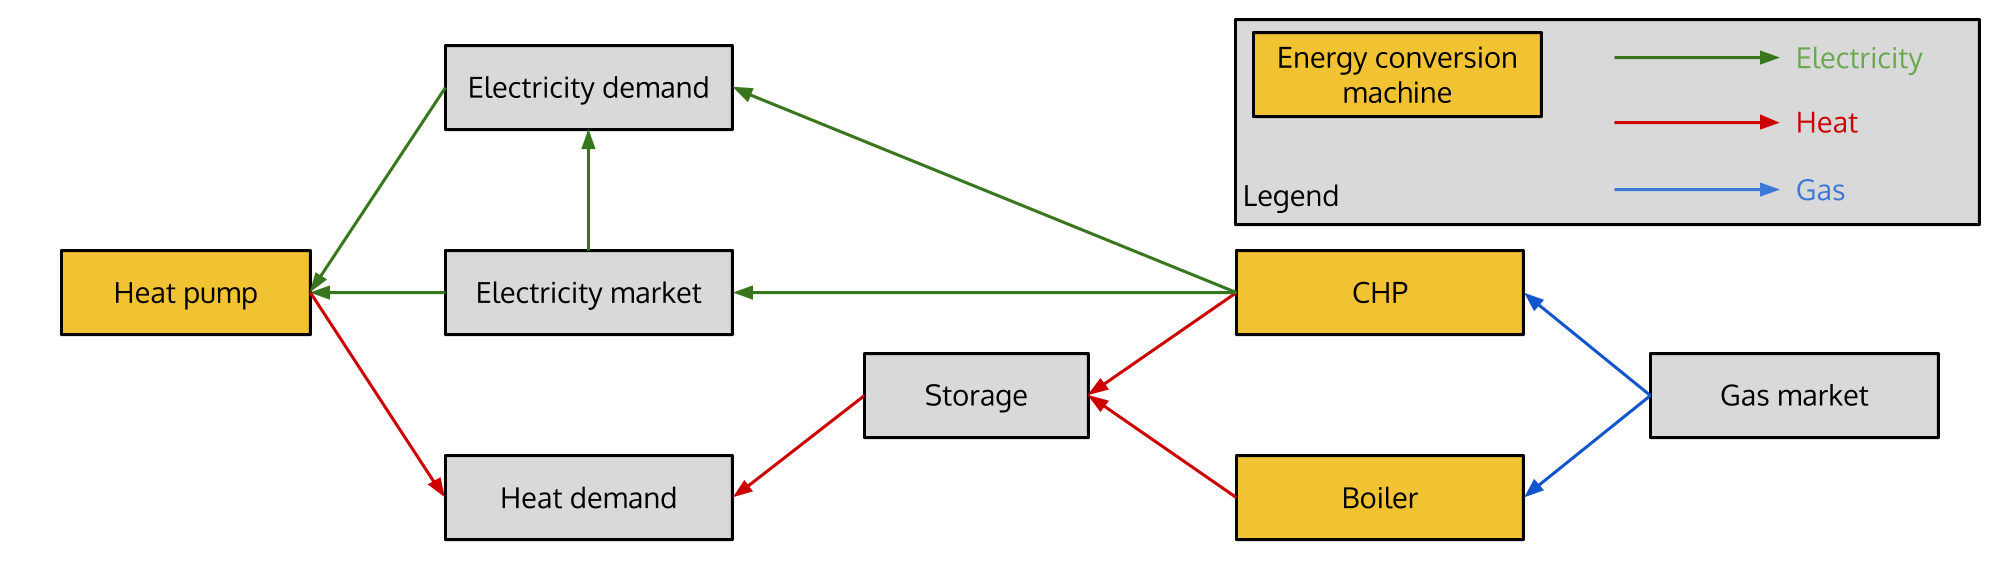
\includegraphics[width=17cm]{Images/FlowchartGeneral.png}}
	\setlength{\fboxsep}{0.1 cm}
	\caption{An overview of the general system model. One can see the different energy streams (electricity, green; heat, red; gas, blue).}
	\label{F:GeneralFlowshart}
\end{figure}

\begin{eqnarray}
\text{Electrical efficiency} &=& \frac{\text{Electrical output} [\unit{kW}]}{\text{Fuel input} [\unit{kW}]}\\
\text{Overall efficiency} &=& \frac{\text{Heat} + \text{Electrical output} [\unit{kW}]}{\text{Fuel input} [\unit{kW}]}
\end{eqnarray}

\chapter{Conclusion}
\label{s:Conclusion}

%\input{General/Conclusion.tex}

\bibliographystyle{plain}
\bibliography{References/Bibliography}
%\bibliographystyle{plain}
\bibliography{References/References}

%\begin{thebibliography}{5}
%\bibitem{cit:Pamadi2}
%
%
%Bandu N. Pamadi,
%Performance, Sability, Dynamics, and Control of Airplanes,
%Second edition,
%American Institute of Aeronautics and Astronautics
%p.294 figure 3.92
%\end{thebibliography}


\end{document}
